\documentclass{article}

% if you need to pass options to natbib, use, e.g.:
% \PassOptionsToPackage{numbers, compress}{natbib}
% before loading nips_2016
%
% to avoid loading the natbib package, add option nonatbib:
% \usepackage[nonatbib]{nips_2016}
\usepackage[final]{nips_2016} % produce camera-ready copy

% to compile a camera-ready version, add the [final] option, e.g.:
% \usepackage[final]{nips_2016}

\usepackage[utf8]{inputenc} % allow utf-8 input
\usepackage[T1]{fontenc}    % use 8-bit T1 fonts
\usepackage{hyperref}       % hyperlinks
\usepackage{url}            % simple URL typesetting
\usepackage{booktabs}       % professional-quality tables
\usepackage{amsfonts}       % blackboard math symbols
\usepackage{nicefrac}       % compact symbols for 1/2, etc.
\usepackage{microtype}      % microtypography

\title{Deep Neural Network based Text-to-Speech
	\\
	Beszédszintézis Mély Neurális Hálóval}

% The \author macro works with any number of authors. There are two
% commands used to separate the names and addresses of multiple
% authors: \And and \AND.
%
% Using \And between authors leaves it to LaTeX to determine where to
% break the lines. Using \AND forces a line break at that point. So,
% if LaTeX puts 3 of 4 authors names on the first line, and the last
% on the second line, try using \AND instead of \And before the third
% author name.

\author{
	Tamas Szanto\\
	\texttt{tmas.szanto@gmail.com} \\
	\AND
	Gergely D. Nemeth\\
	\texttt{NeGeD.NG@gmail.com} \\
}

\begin{document}
% \nipsfinalcopy is no longer used

\maketitle
\chapter{}
\begin{abstract}
  Human-like communication with the computers is a major application of Computer Science. The Text-to-Speech methods are significant part of the project. This paper is a review of the authors experience about the usefulness of the Deep Neural Networks' new fields regarding to the \textbf{TTS} problem.
\end{abstract}

\begin{abstract}
	A Számítástechinka egyik meghatározó célja a számítógépekkel való emberszerű kommunikáció elérése. A Beszédszintézis ennek elengedhetetlen területe. Jelen dokumentum a szerzők a Mély Neurális Hálók nyújtotta lehetőségek a témában való alkalazásából szerzett tapasztalatainak összefoglalója. 
\end{abstract}

\clearpage

\chapter{}
\section{WaveNet tapasztalatok}

Első célnak a beszédszintézis WaveNet[1] alapú megoldását tűztük ki. Ennek lényege az aktuális időpillanatban a hanghullám értékénék az előző, már meghatározott értékek és a szövegfeldolgozásból kapott címkék segítségével történő meghatározása. Két rendszertervet dolgoztunk ki, azzal a különbséggel hogy a fonéma hosszának a becslése egy külön hálóban történik vagy a kimenetről van visszavezetve. Utóbbi esetben a hullámérték mellett lenne egy másik kimeneti érték is, amely azt adná meg hogy kezdődjön-e az új fonéma.

\begin{centering}
	\textbf{WaveNet külön fonéma becsült hálóval}\par\medskip\centering
	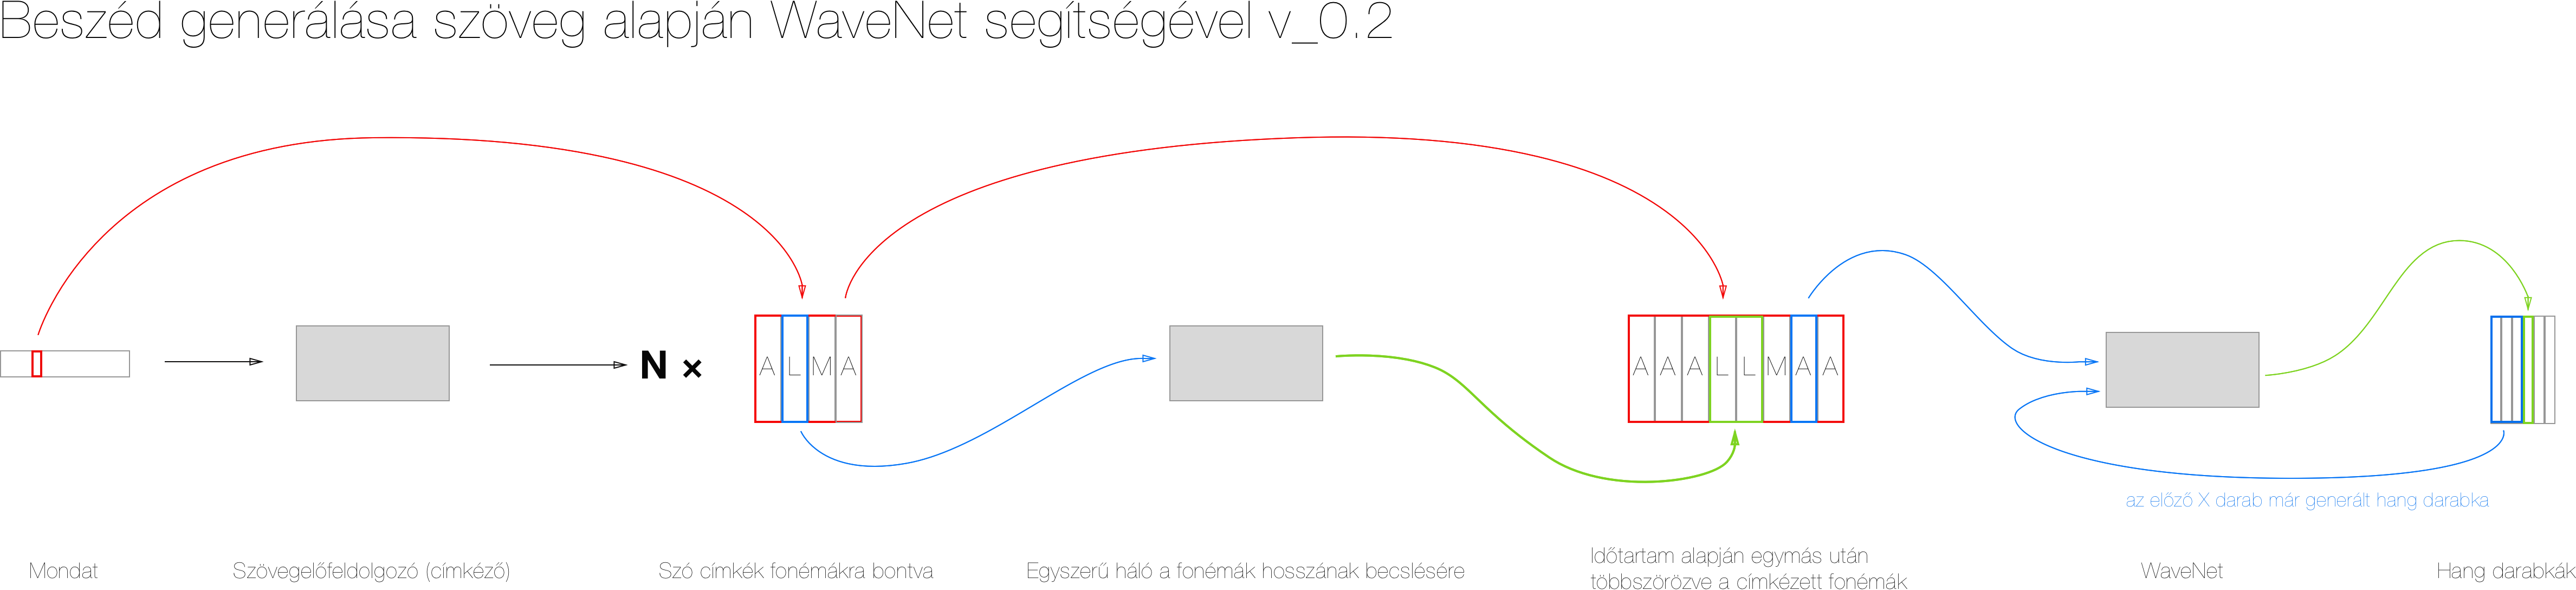
\includegraphics[width=\textwidth,keepaspectratio]{wavenet_0_2}
	
	\textbf{WaveNet fonéma becsléssel kiegészítve}\par\medskip
	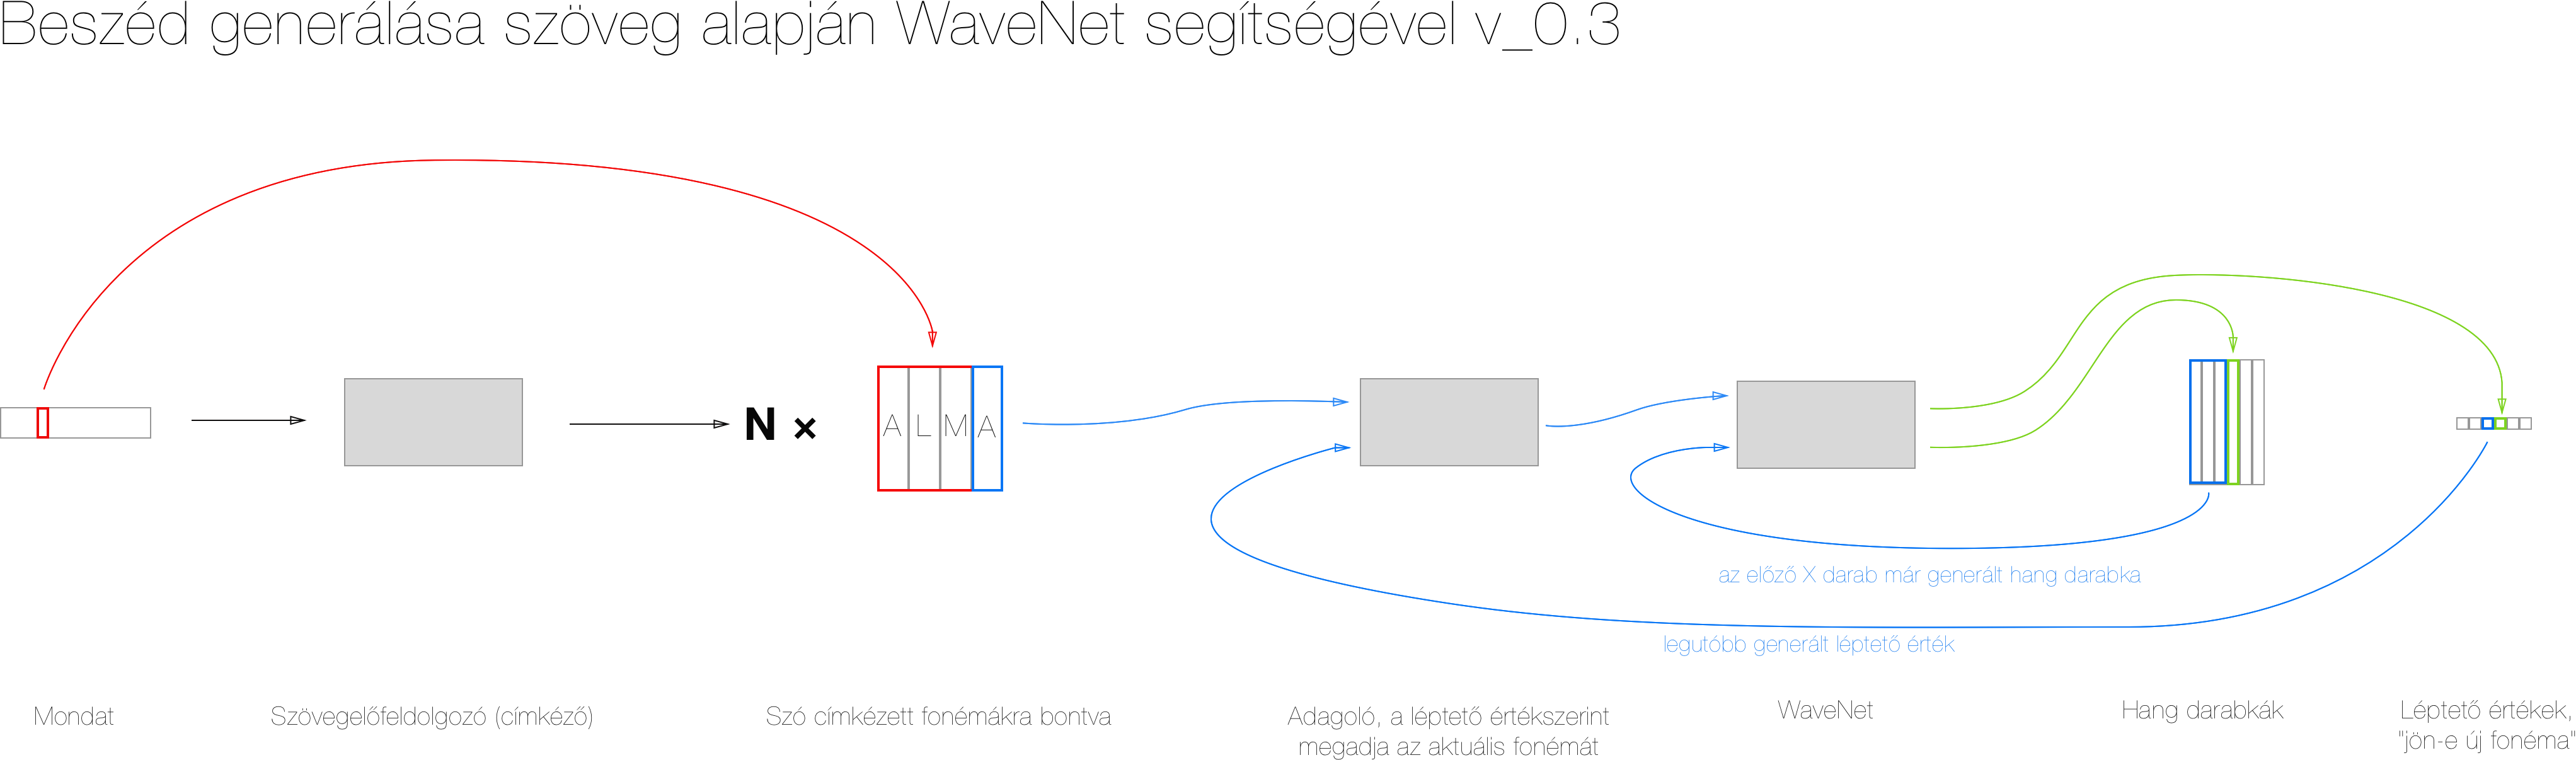
\includegraphics[width=\textwidth,keepaspectratio]{wavenet_0_3}
\end{centering}

A megvalósítás során először már meglévő, GitHub-on elérhető implementációkat próbáltunk ki. Ezek közül az egyiket sikerült egy adott mondatra tanítanunk, azt vissza tudta generálni pontosan. Azonban más mondatokkal való továbbtanítás esetén már nem volt működőképes.

Ezután saját implementációval próbálkoztunk a DeepMind által publikált cikk alapján. Ez az implementáció lényegesen egyszerűbb volt mint a cikkben meghatározott, célunk csak valamilyen kis zörej előállítása volt. Azonban konstans (néma) hangon kívül mást nem sikerült előállítanunk.

A fent említett kísérletek után egyértelművé vált, hogy túl nagy feladatba kezdtünk bele. Ezért visszaléptünk az eredeti célunktól és folytatásképpen a hagyományos DNN alapú beszédszintézissel haladtunk tovább.
\chapter{}
\section{Egyszerű DNN model felépítése}
\label{dnn_model}
A továbbiakban egy DNN model alkalmazása olvasható. A megismert cimkéket továbbiakkal egészítettük ki, majd ez alapján generáltunk gerjesztési és spektrális paramétereket, amikből előállítható az audio.

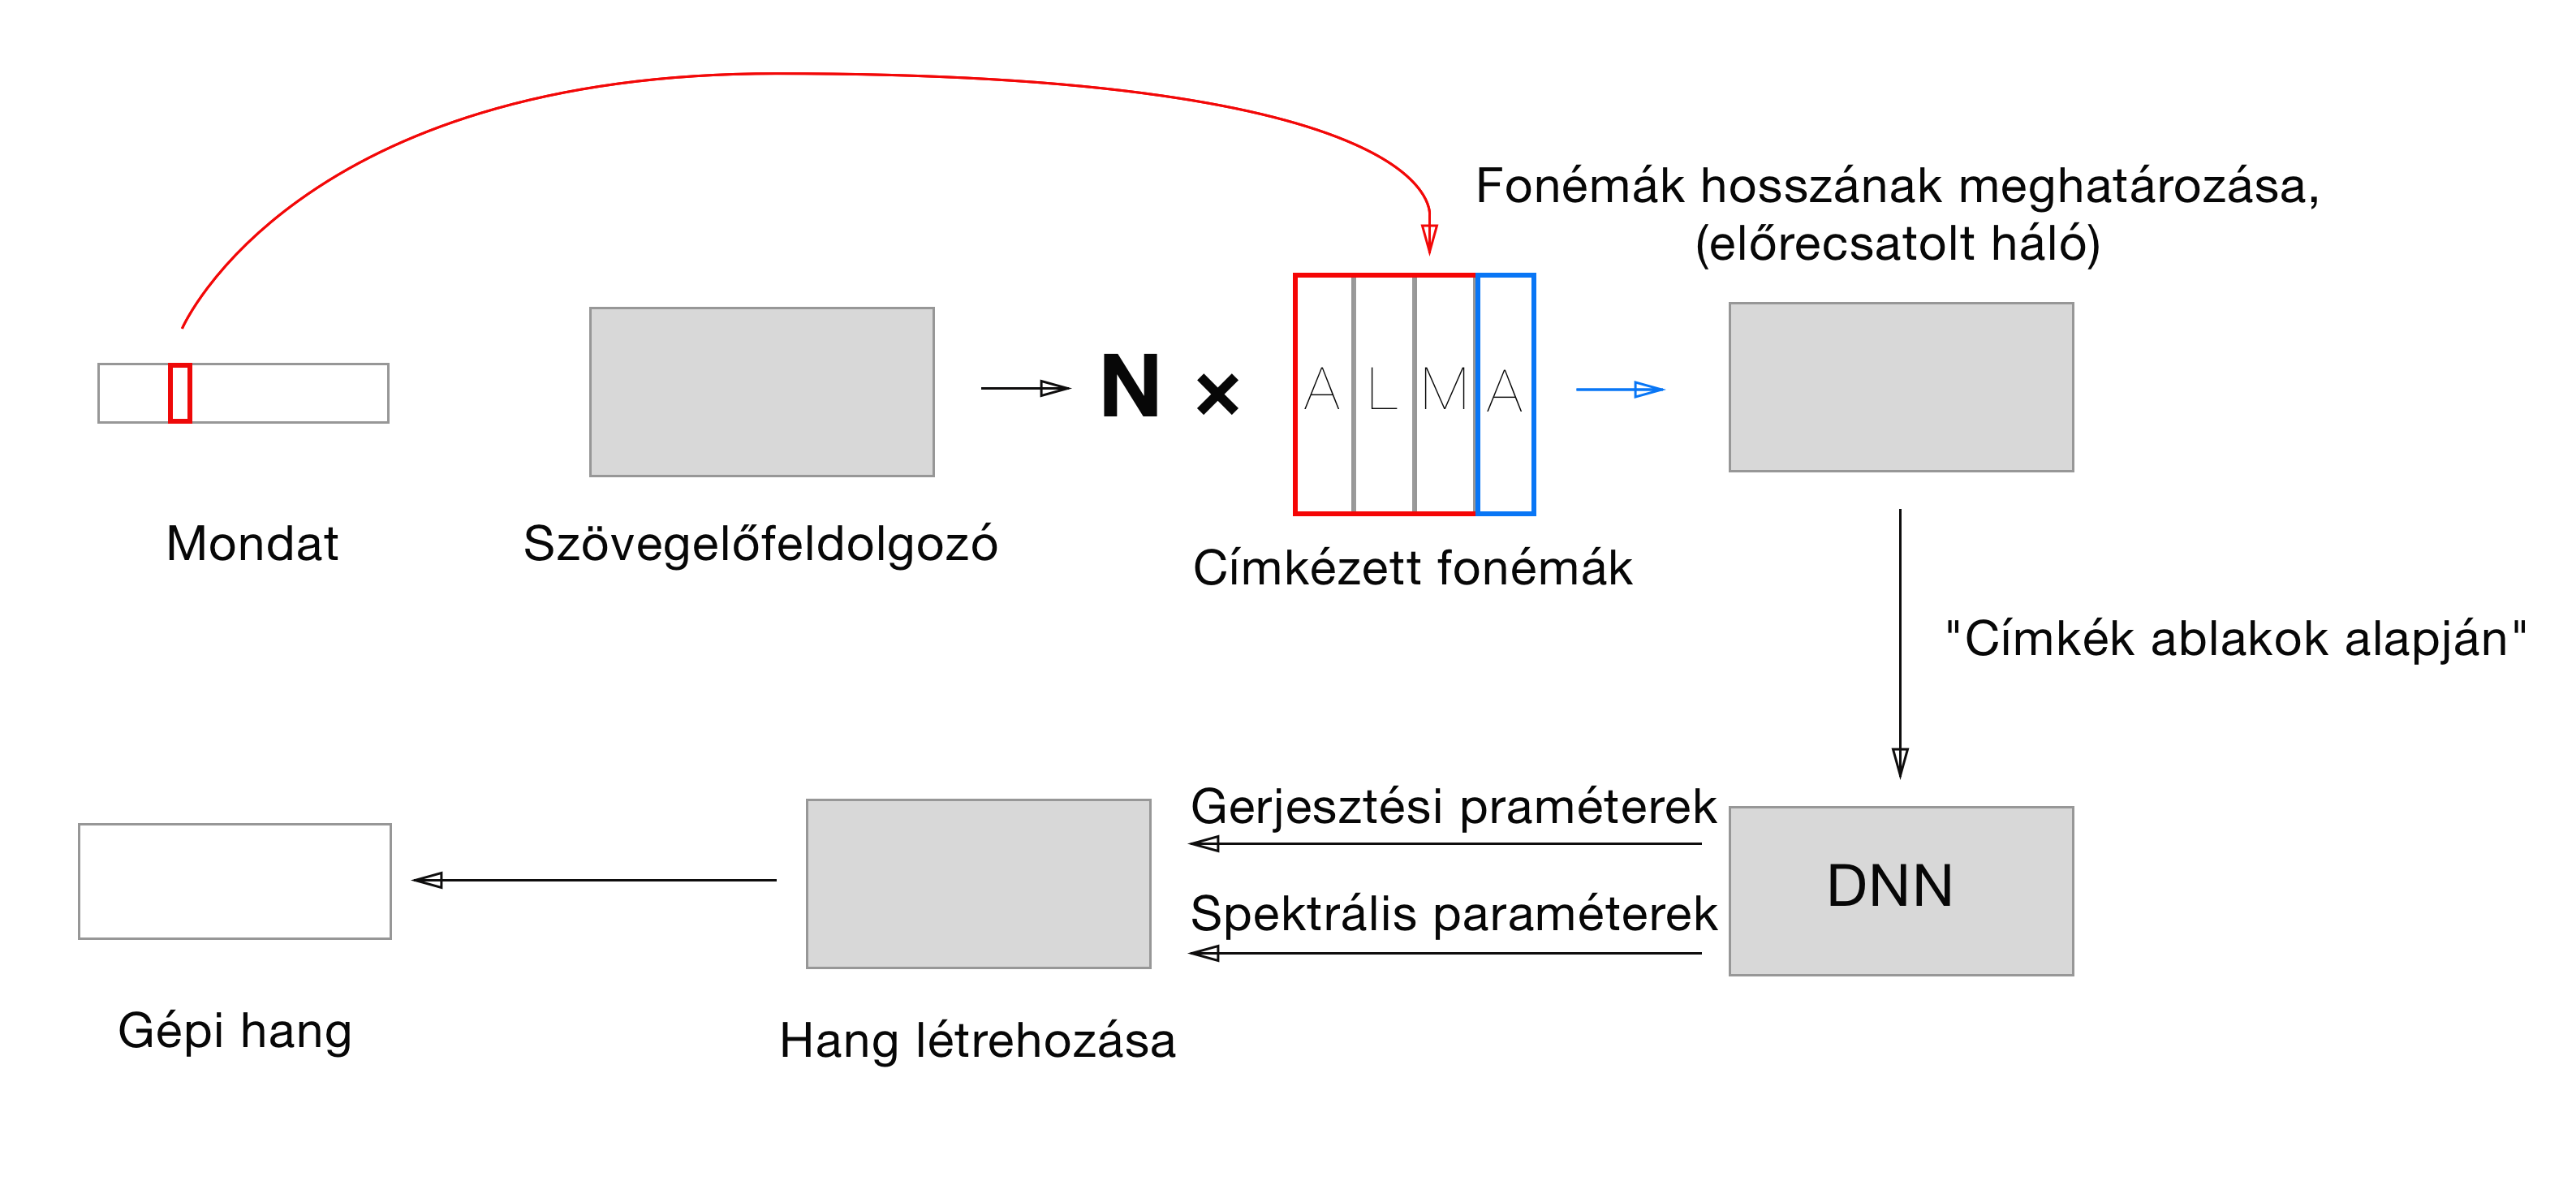
\includegraphics[width=\textwidth,keepaspectratio]{dnn_struct}

\subsection{Háló modell}
Külön hálón tanítottuk a spektrális és a gerjesztési paramétereket. 

Előrecsatolt mély neurális hálózatot építettünk fel, 6 rejtett réteggel, tanh és sigmoid aktivációs függvényekkel, SGD optimalizálóval és MSE költségfüggvénnyel. A háló rétegeire Dropoutot is használtunk. (/!TODO ref)
A megállást early stoppinggal detektáltuk.

/!TODO háló modell kép
\chapter{}
\subsection{Bemeneti és kimeneti paraméterek}
\subsubsection{One Hot kódolás}
A fonéma azonosítására az OneHot kódolást alkalmaztuk (/!TODO referencia), azaz minden fonémára 40 paramétert generáltunk. A már megismert fonéma cimkéket kiegészítettük a fonémában található keretek számával és a keret fonémán belüli elhelyezkedésével, így a kerethez tartozó 215 bemeneti paraméter az alábbiakból tevődik össze:
\subsubsection{Bemeneti paraméterek}
\begin{minipage}{0.5\textwidth}
\begin{itemize}
	\item 0-200 A 40 paraméter a kvinfónra(2-1-2)
	\item 200-213 Fonéma cimkék
	\item 213 A fonémán belüli keretek száma
	\item 214 A keret elhelyezkedése a fonémán belül
\end{itemize} 
\end{minipage} \hfill
\begin{minipage}{0.5\textwidth}
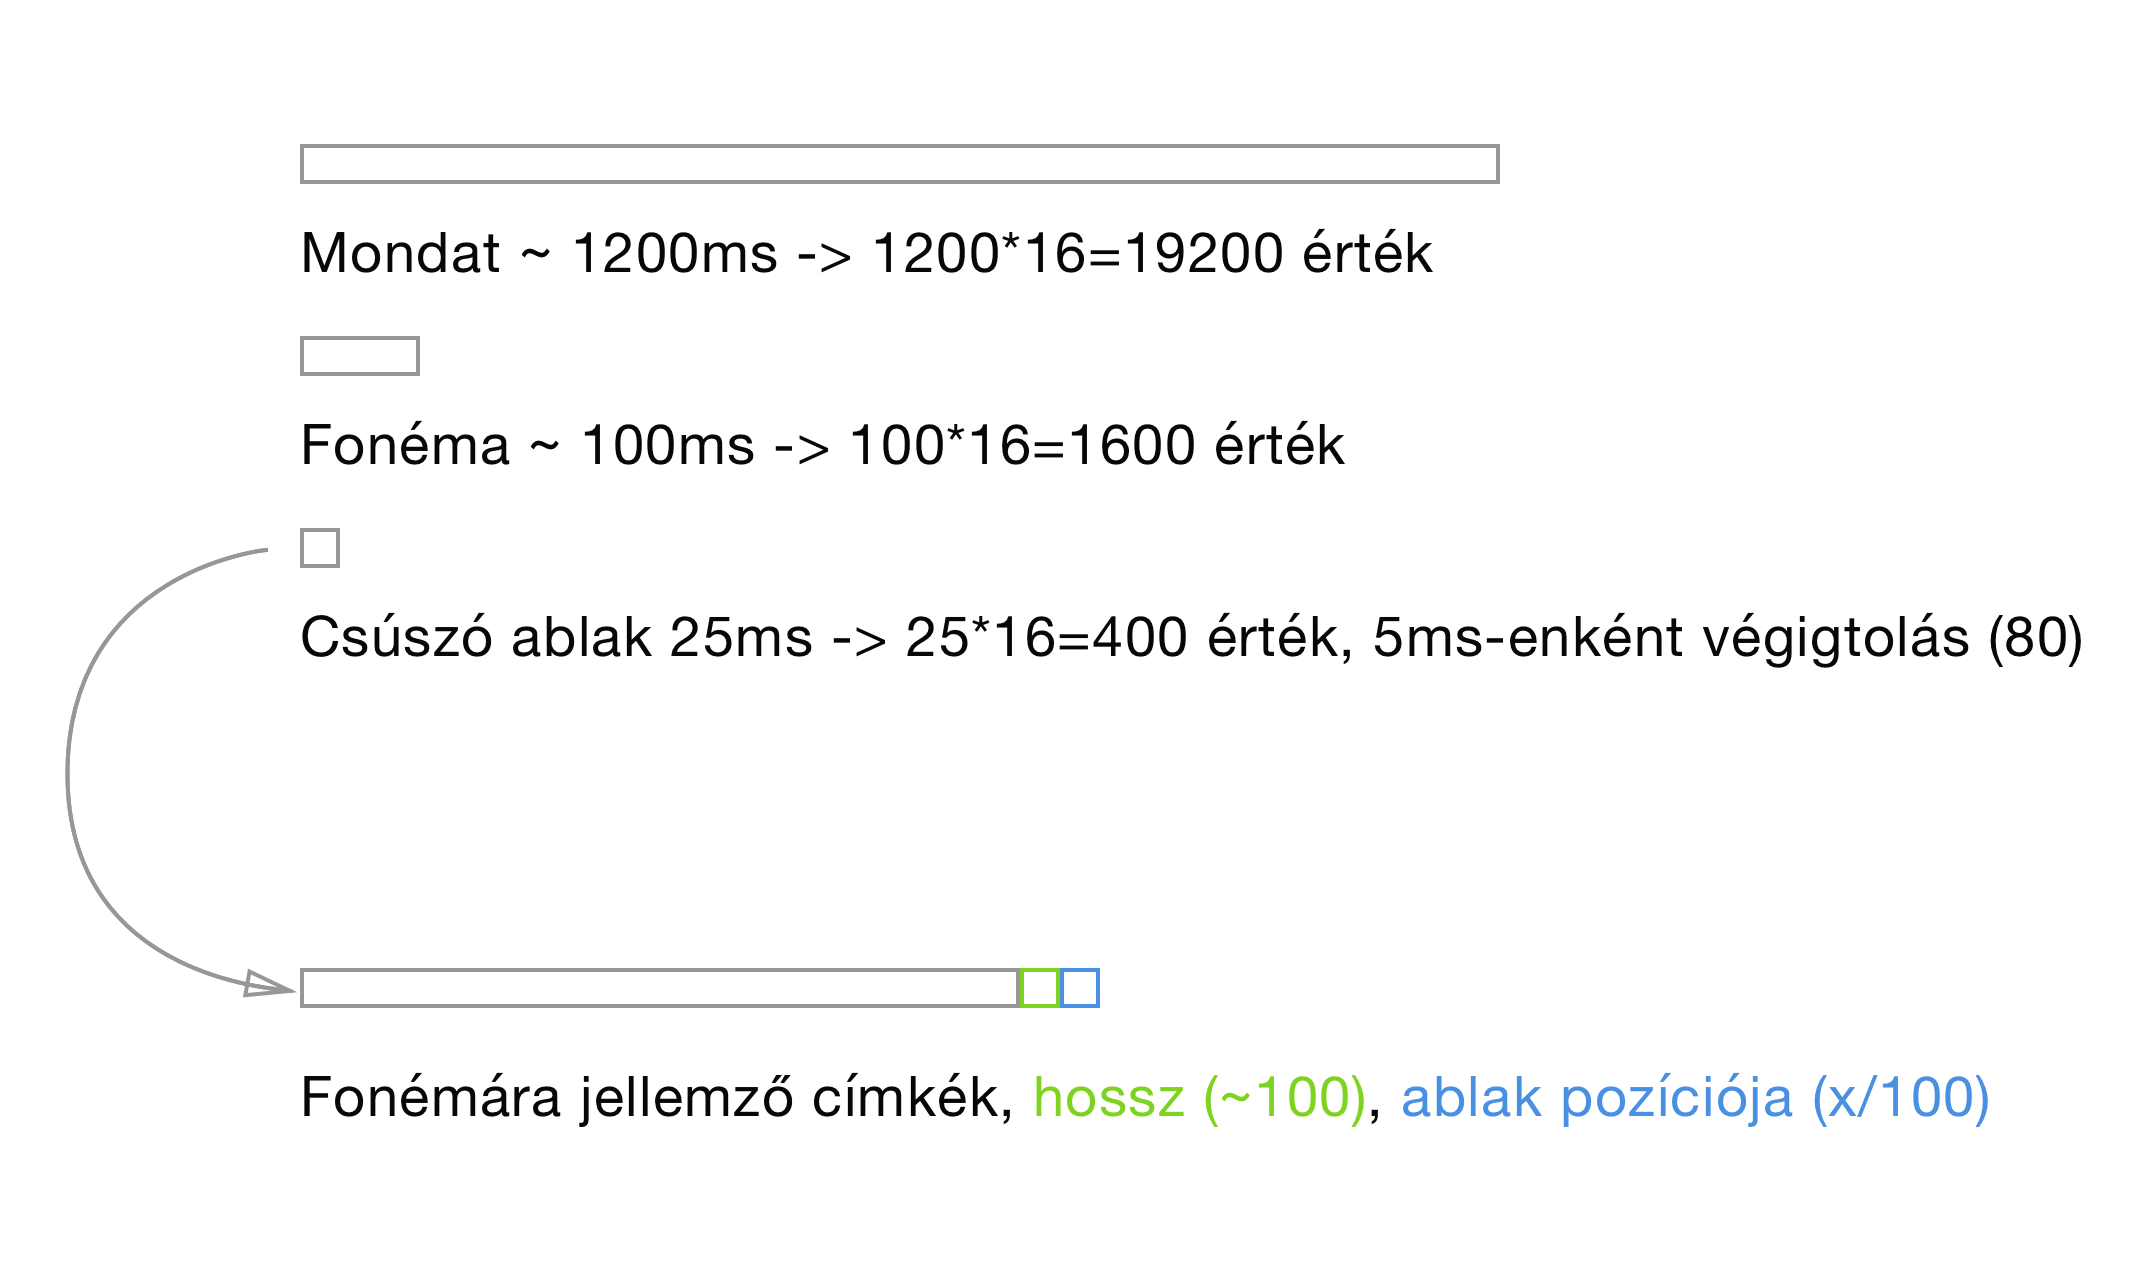
\includegraphics[width=5.5cm,keepaspectratio]{tag_struct}
\end{minipage} \hfill
\subsubsection{Kimeneti paraméterek}
\begin{itemize}
	\item 215 a keret hangmagasság értéke
	\item 216-242 a Mel-Cepstrum 26 paramétere
	\item 242 a fonémán belüli keretek száma
\end{itemize}
\subsection{Spektrális és gerjesztési paraméterek}
Mint említettük a prediktálás alapja a spektrális és gerjesztési paraméterek megadása keretenként. Ezen paraméterek segítségével a PyPSTK (/!TODO ref) python csomag használásával állíthatjuk elő az audio kimenetet, valamint hasonlóképpen ezt a csomagot használjuk az adataink a tiszta hangból való előállítására.
\subsubsection{Mel-Cepstrum}
A paraméterek előállításához, visszafejtéséhez a PyPSTK Mel-Cepstrum alapú algoritmusát alkalmazzuk. Az algoritmust T. Fukada és társai fejlesztették ki.\ [1]

Ezzel a metódussal természetesen adatvesztést kapunk, azonban az így előállított hang még megfelel a mércéinknek. Viszont az általunk generált kimenetek értékelésénél ezt figyelembe kell vennünk.

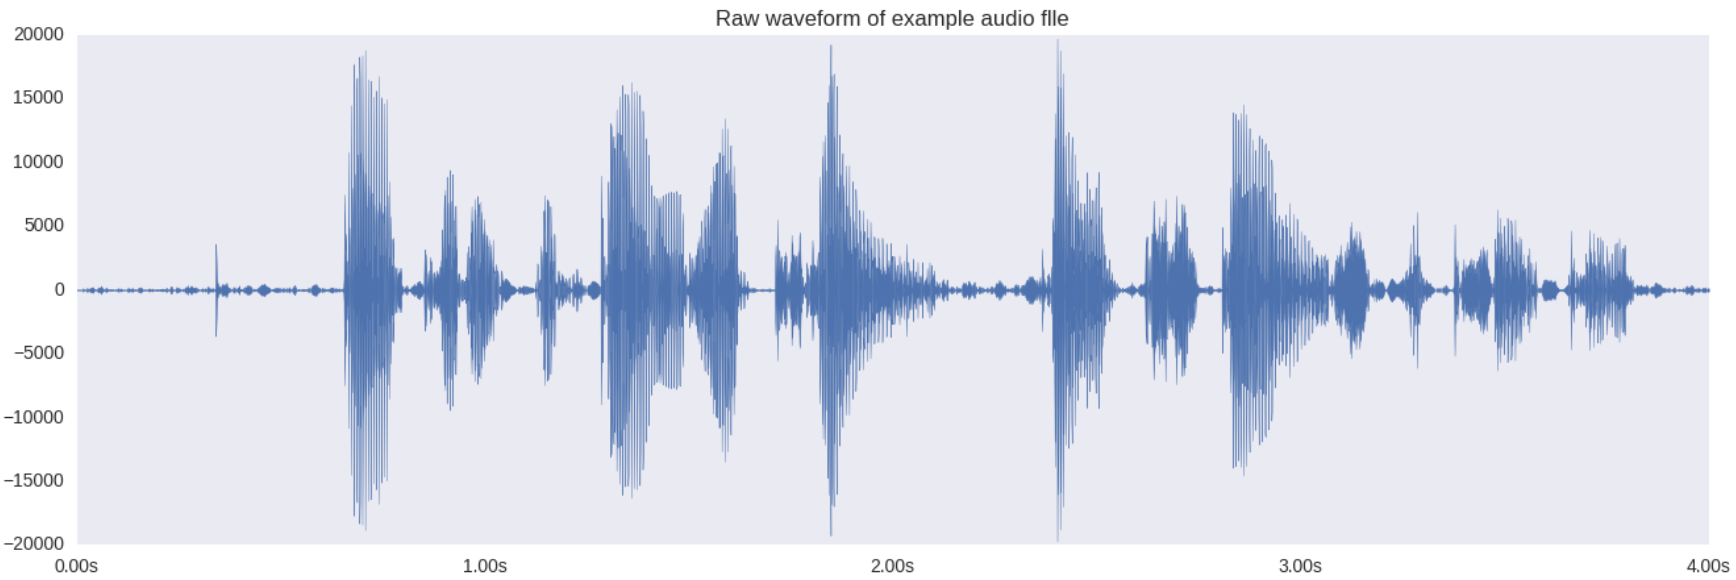
\includegraphics[width=\textwidth,keepaspectratio]{audio_raw}

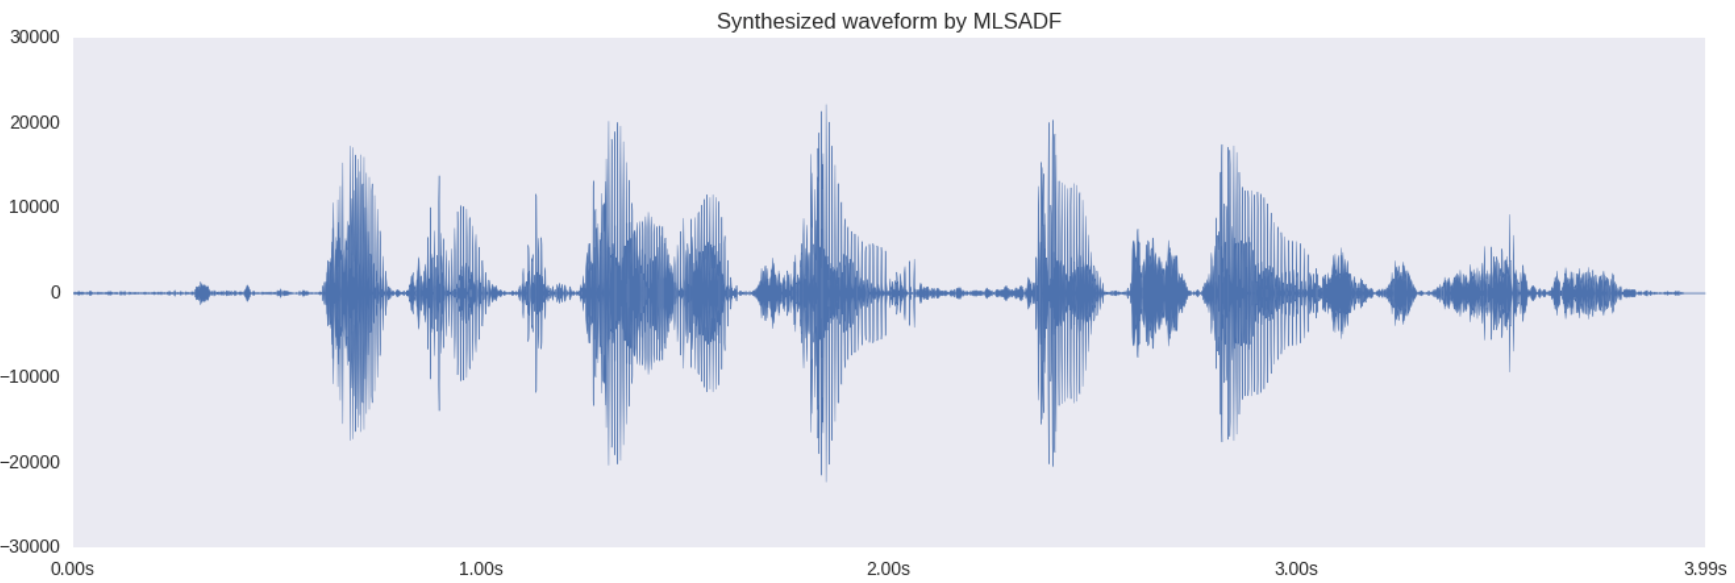
\includegraphics[width=\textwidth,keepaspectratio]{audio_mc}
\chapter{}
\section{Megvalósítás}
\subsection{Használt erőforrások}
A háló összerakást saját gépen kezdtük el. Majd a véglegesítését és a tanításokat AWS szerveren, NVIDIA Tesla K80 12GB videokártyán végeztük. Jupyter notebook-ban futtatuk a tanításokat, kerasban felépített hálóval\ [5], ezek elmentett adatait aztán Tensorboard segítségével elemeztük\ [7].
\subsection{Fejlesztés}
A fejlesztés során scriptet írtunk az adatok generálására( {\it generate\_dataset.py}). Ez állítja elő a tiszta adatfájlokból a hálók bemeneteit.

A különböző hálókat jupyter notebookokban teszteltük. Ezek a {\it model} kezdetű notebookokban találhatóak.

A végső eredményeket a {\it results} notebookban összegeztük, ez végigfuttatható demonstrációként hamar előáll. 
\subsection{Eredmények}
Zöngésség becslésére nagyon jó, alapfrekvencia (pitch érték) meghatározására használhatóan jó és a spektrális paraméter (Mel-Cepstrum) jósolására kezdetleges eredményeket sikerült elérnünk. (utóbbiról ezért nem is mellékeltünk tanítási és validációs grafikonokat). Hiperparaméter optimalizálás tekintetében egyelőre kézzel dolgoztunk (ez még javításra szorul), már így is sikerült használható pontosságot  elérnünk.

\textit{(A grafikonok y tengelyén az MSE hiba értéke x tengelyén az elvégzett epoch-ok száma látható.)}

\subsubsection{Zöngésség}
	Zöngésség becslése egyszerűbb, futásidő tekintetében gyorsabb feladatnak bizonyult. Ezért itt nem alkalmaztunk early stopping-ot, hanem a több próbálkozás után a fixen 410 epoch-kal történő tanításnál maradtunk.
	
	A teszt adatainkon elért eredmények:
	
	pontosság 0.8342
	
	költségfüggvény: 0.1560
	
	\textit{(MSE hiba értékekkel számítva)}

\begin{figure}[h]
	\par\centering
	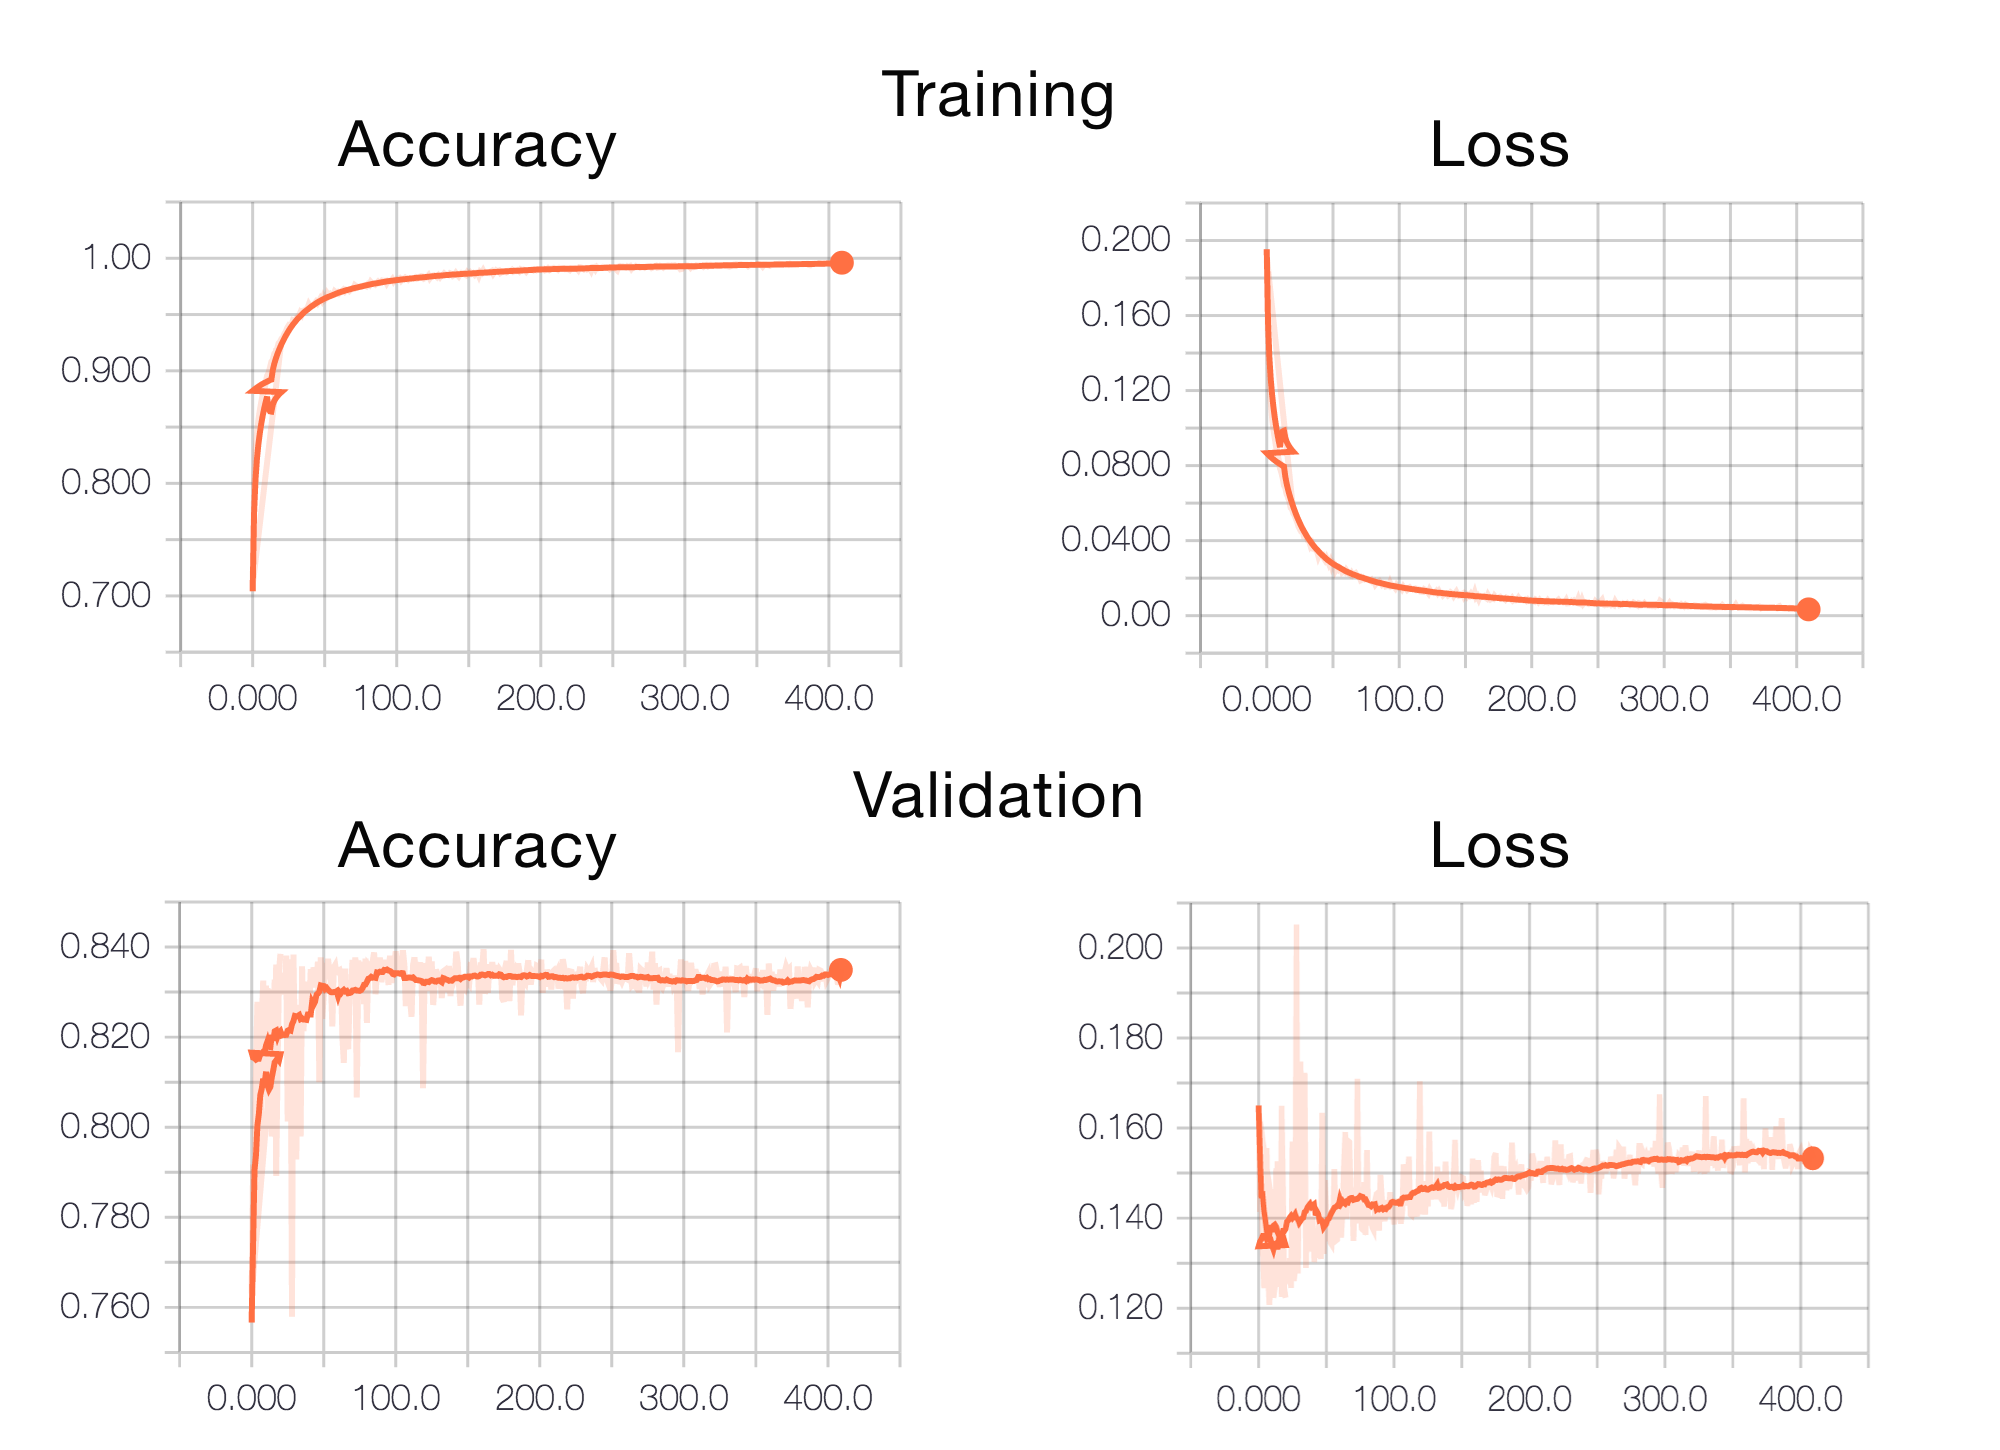
\includegraphics[width=0.65\textwidth,keepaspectratio]{uv_fig}
	\caption{Zöngésség tanítás}
\end{figure}

\subsubsection{Alapfrekvencia}
Az alapfrekvencia tanítása esetén alkalmaztunk early stoppig-ot. Ez azonban (a paramétereinek állítása után is) túl hamar állt meg. Ennek következtében több tanítást is elvégeztünk egymás után. Az itt kapott eredményeink messze nem olyan szépek mint a zöngésségé, de ezek is használhatónak bizonyultak.

A teszt adatainkon elért eredmények:

pontosság: 0.4243

költségfüggvény: 0.07214

\textit{(MSE hiba értékekkel számítva)}
\begin{figure}[h]
	\par\centering
	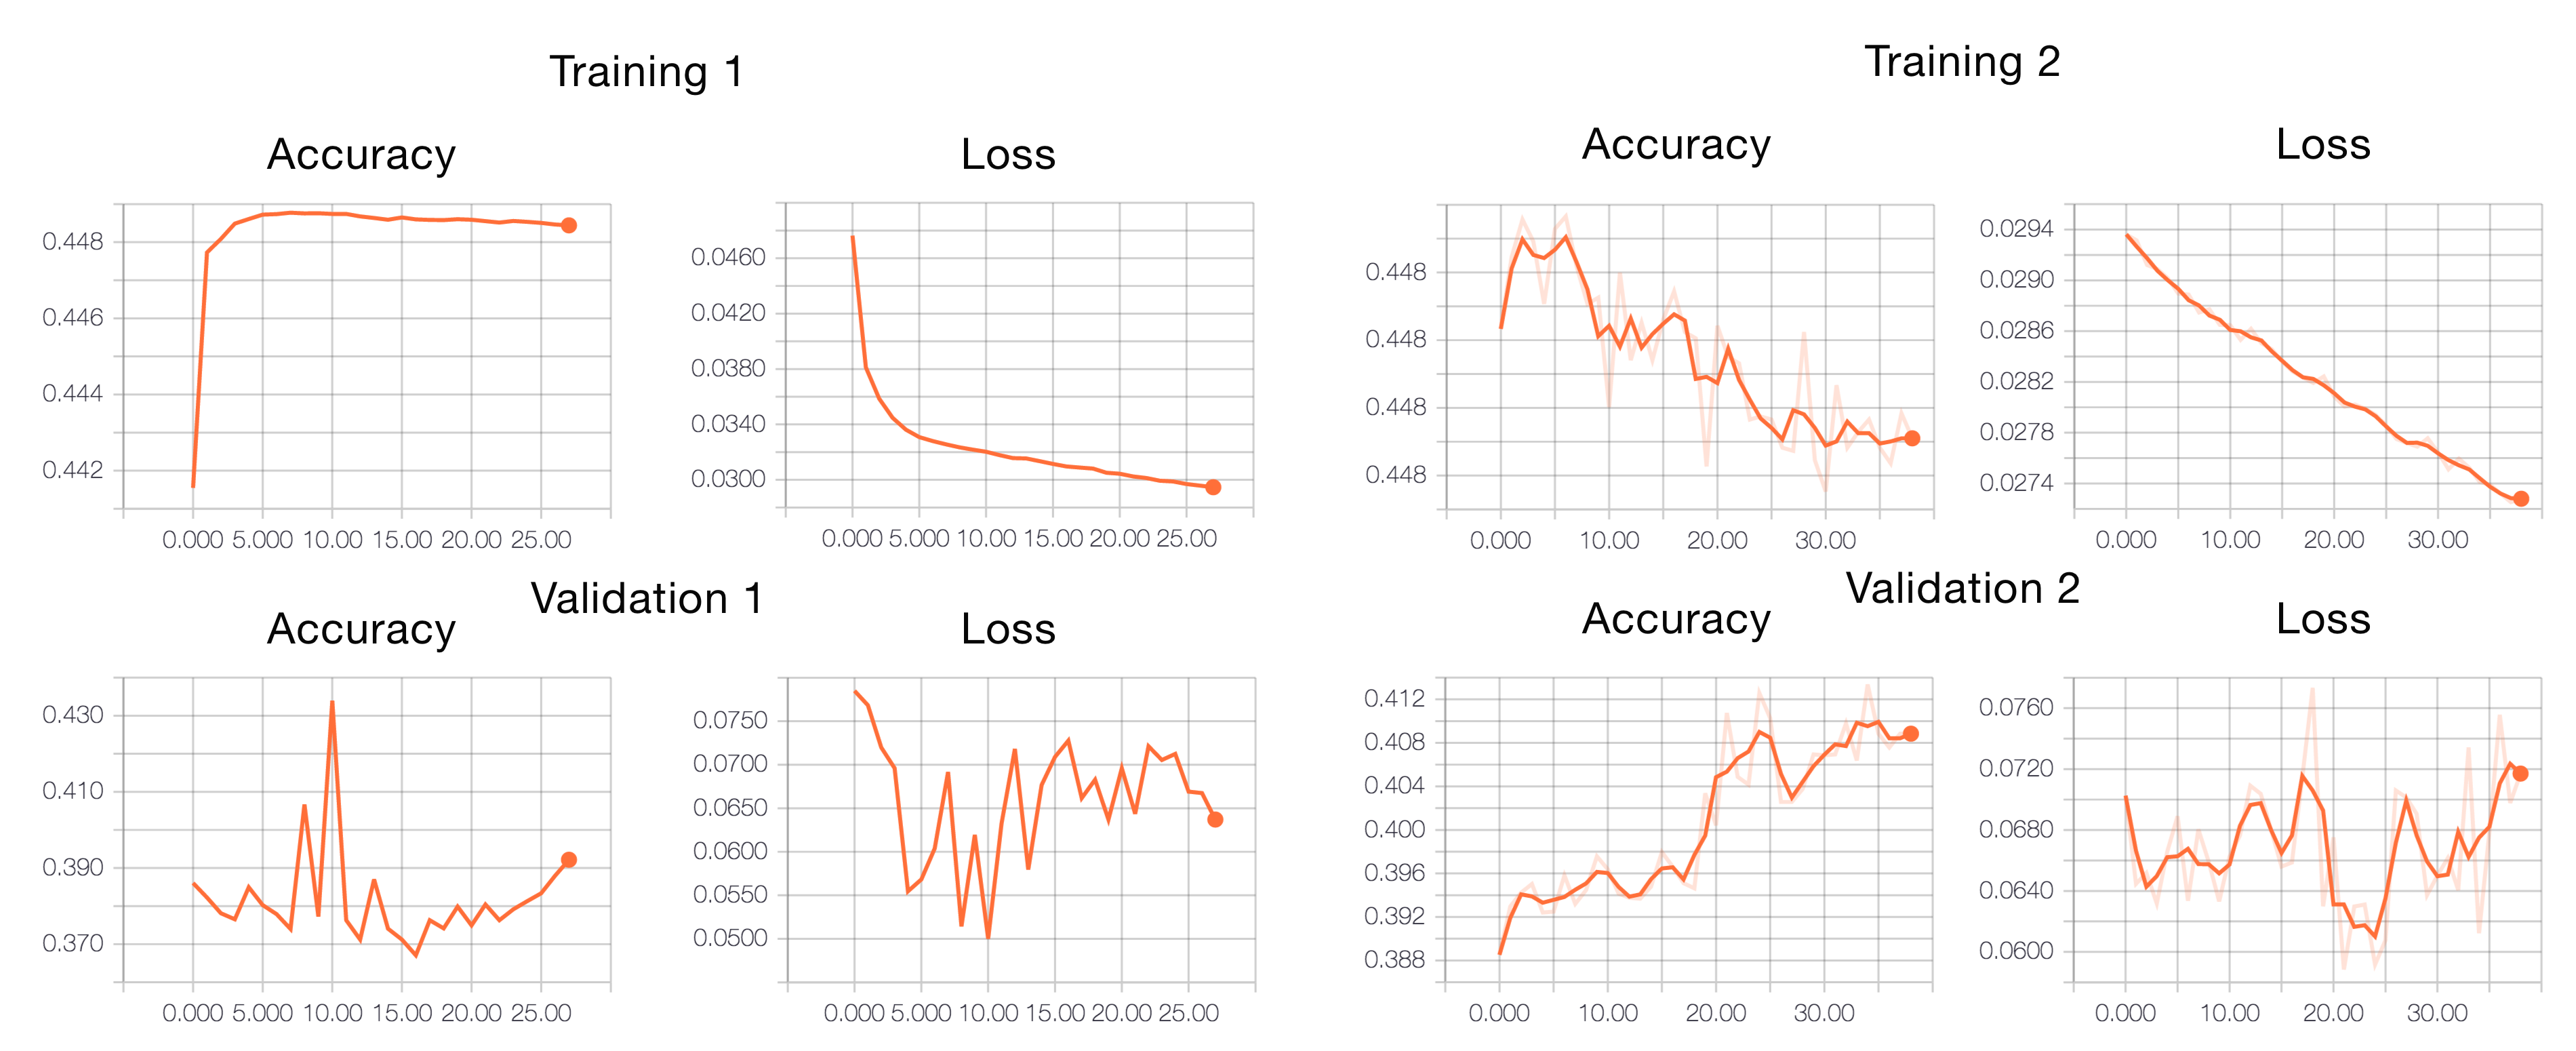
\includegraphics[width=\textwidth,keepaspectratio]{pitch_fig}
	\caption{Pitch tanítás}
\end{figure}
\subsubsection{MC paraméterek}
MC tanításakor kiütközött, hogy a bemeneti paramétereink nagyon megegyezőek voltak fonémán belül, így darabos lett a tanítás. Ez a magasabb MC értékekre jelentős hibát okozott, így megpróbáltuk kevesebb mc érték használatát pontosítani.

	
	A teszt adatainkon elért eredmények:
	
	pontosság 0.2927
	
	költségfüggvény: 0.2086
	
	\textit{(MSE hiba értékekkel számítva)}
\begin{comment}
Innen hiányzik egy kép
\begin{figure}[h]
	\par\centering
	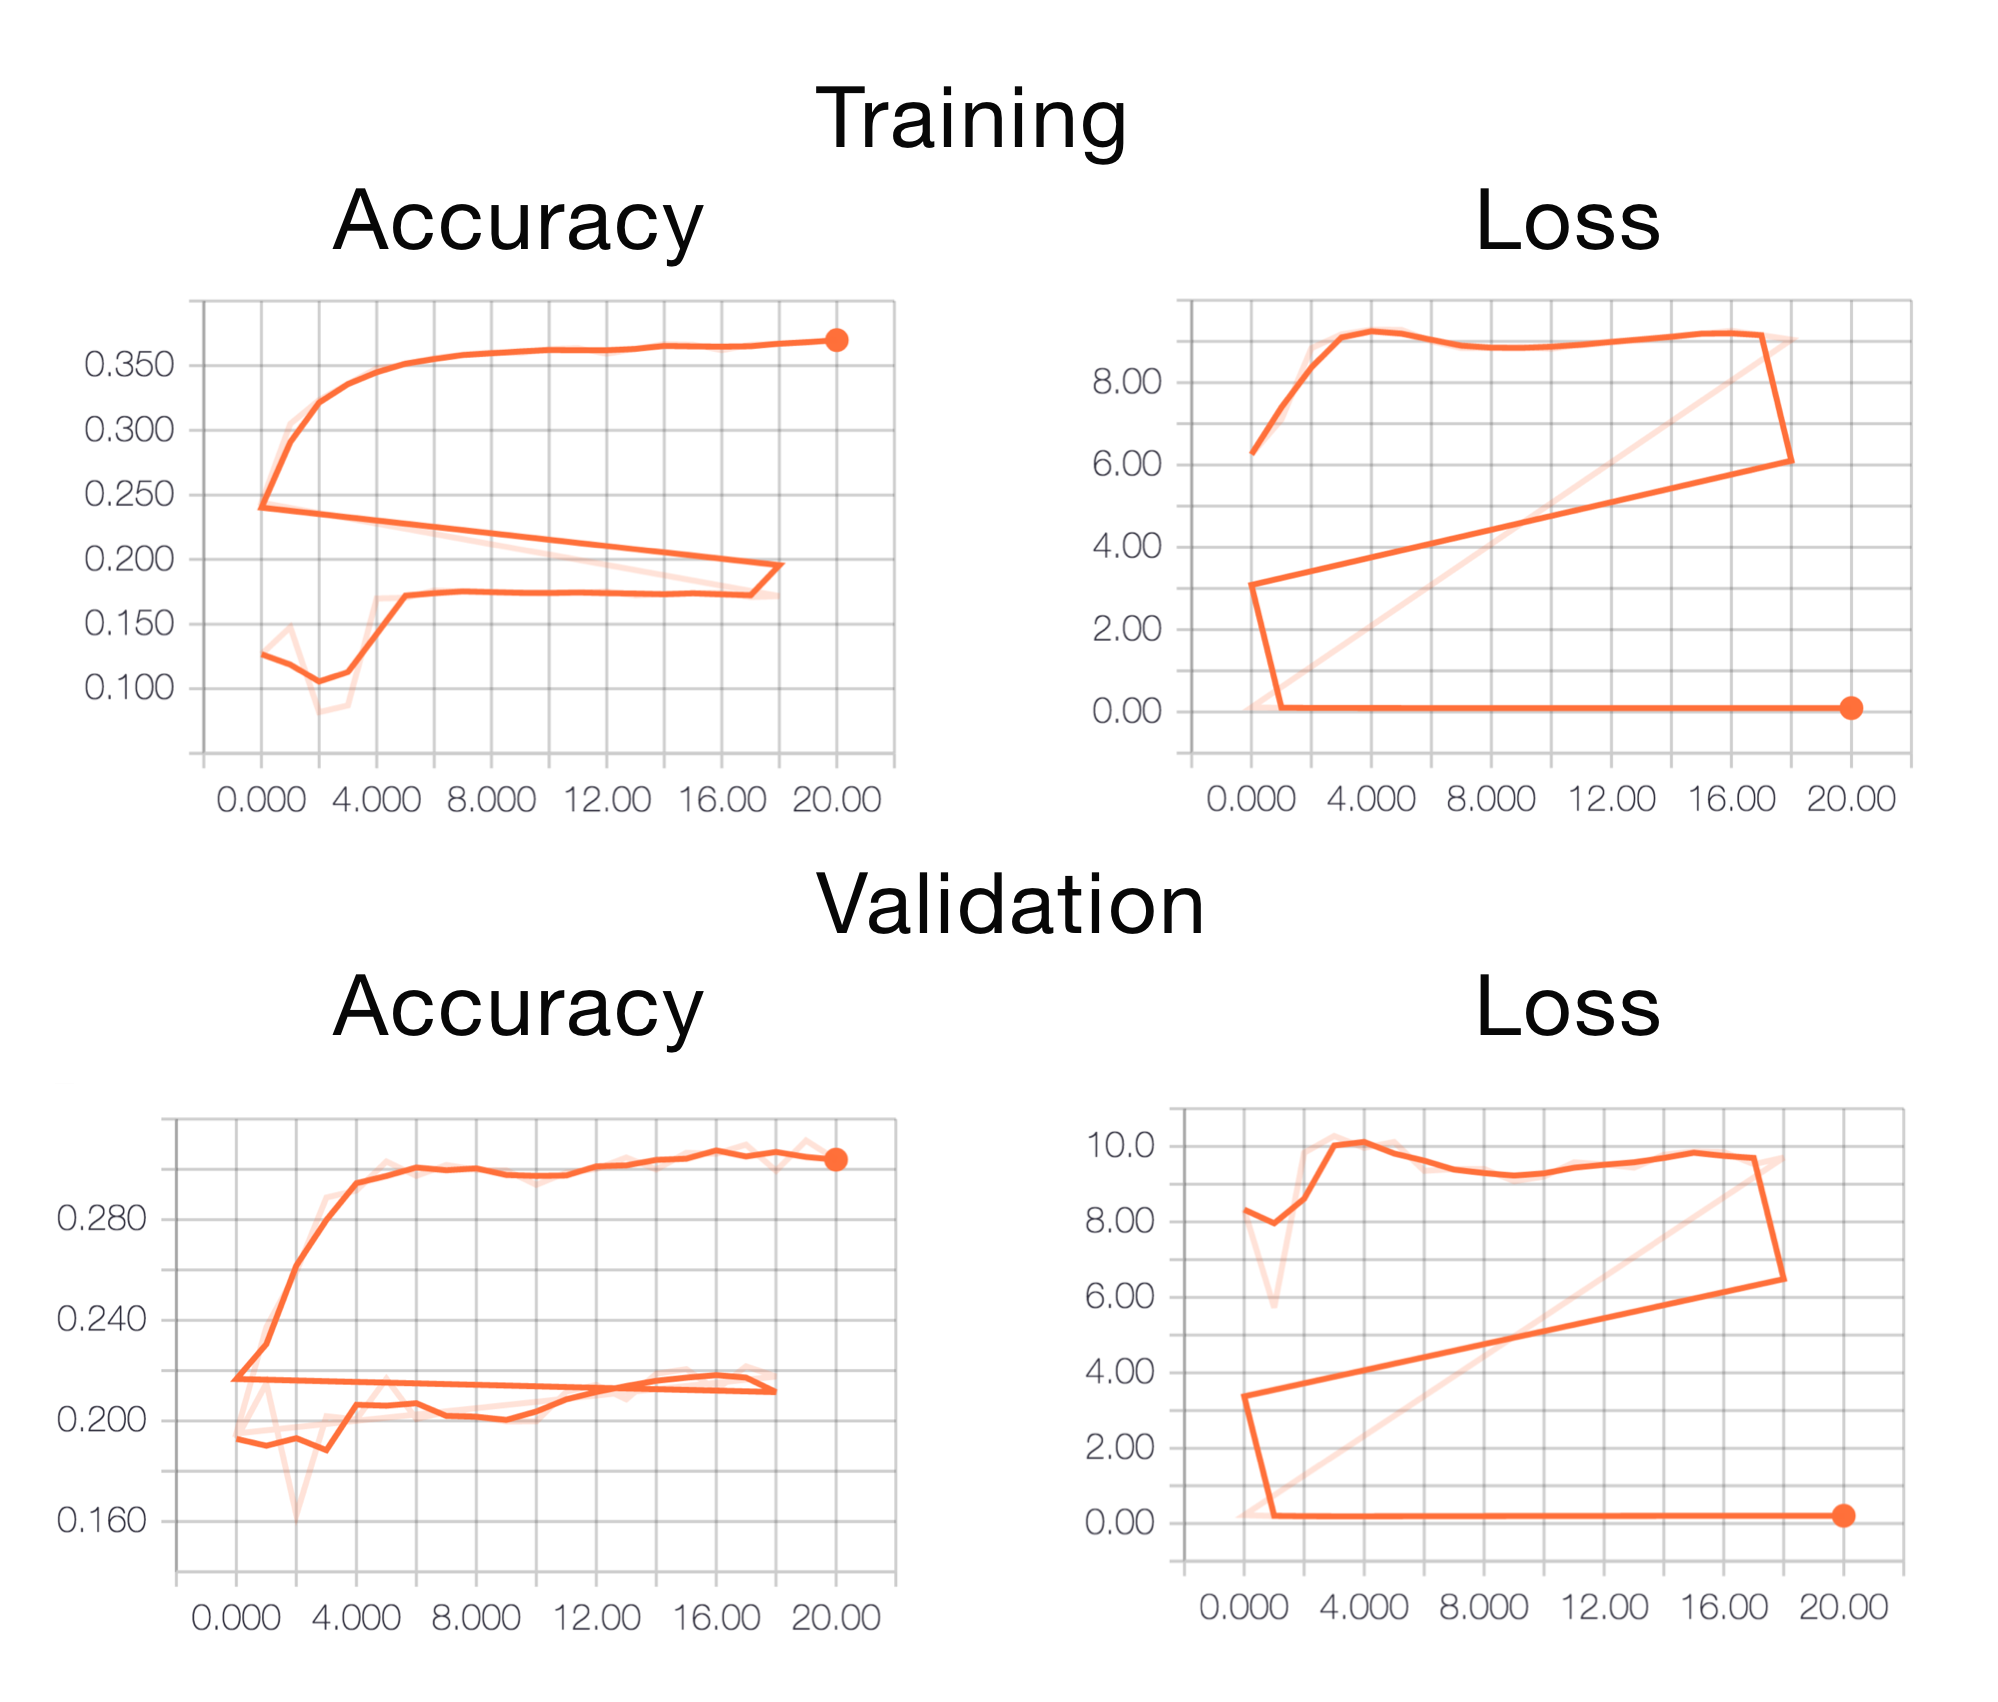
\includegraphics[width=0.8\textwidth,keepaspectratio]{length_fig}
	\caption{MC paraméterek tanítása}
\end{figure}
\end{comment}
\subsubsection{Fonéma hossz}
Fonéma hossz becslésnél csoportosítást valósítottunk meg, a fonémákat 8 csoportba osztottuk, a csoportok között 12,5 ms eltéréssel és a csoportra végeztünk classificationt. Erre azért volt szükség mivel viszonylag kevés, géppel annotált tanító adat állt a rendelkezésünkre, ezek alapján nem sikerült használható eredményeket elérni(1000 mondat, kb. 16000 fonéma ami átlagosan egy fonémára 400 mintát jelent, de ez nem egyenletes így előfordulhat olyan fonéma amire ennél jóval kevesebb tanítóadat szerepel). 

Az adatokban szereplő eredeti hosszak vizsgálata után ezt a csoportosítási módot választottuk, két szempont a megfelelő differenciálódás és a jelentősen kilógó adatok levágása volt. Tehát minden fonémánk 40 és 140 ms közé került. (A tanító adatainkat is ez alapján módosítottuk még a feldolgozási fázisban, minden keretnél hosszabb fonémát 140 ms-nél levágunk.)


A teszt adatainkon elért eredmények:
	
pontosság 0.4619
	
költségfüggvény: 0.02419
	
\textit{(MSE hiba értékekkel számítva)}

\begin{figure}[h]
	\par\centering	
	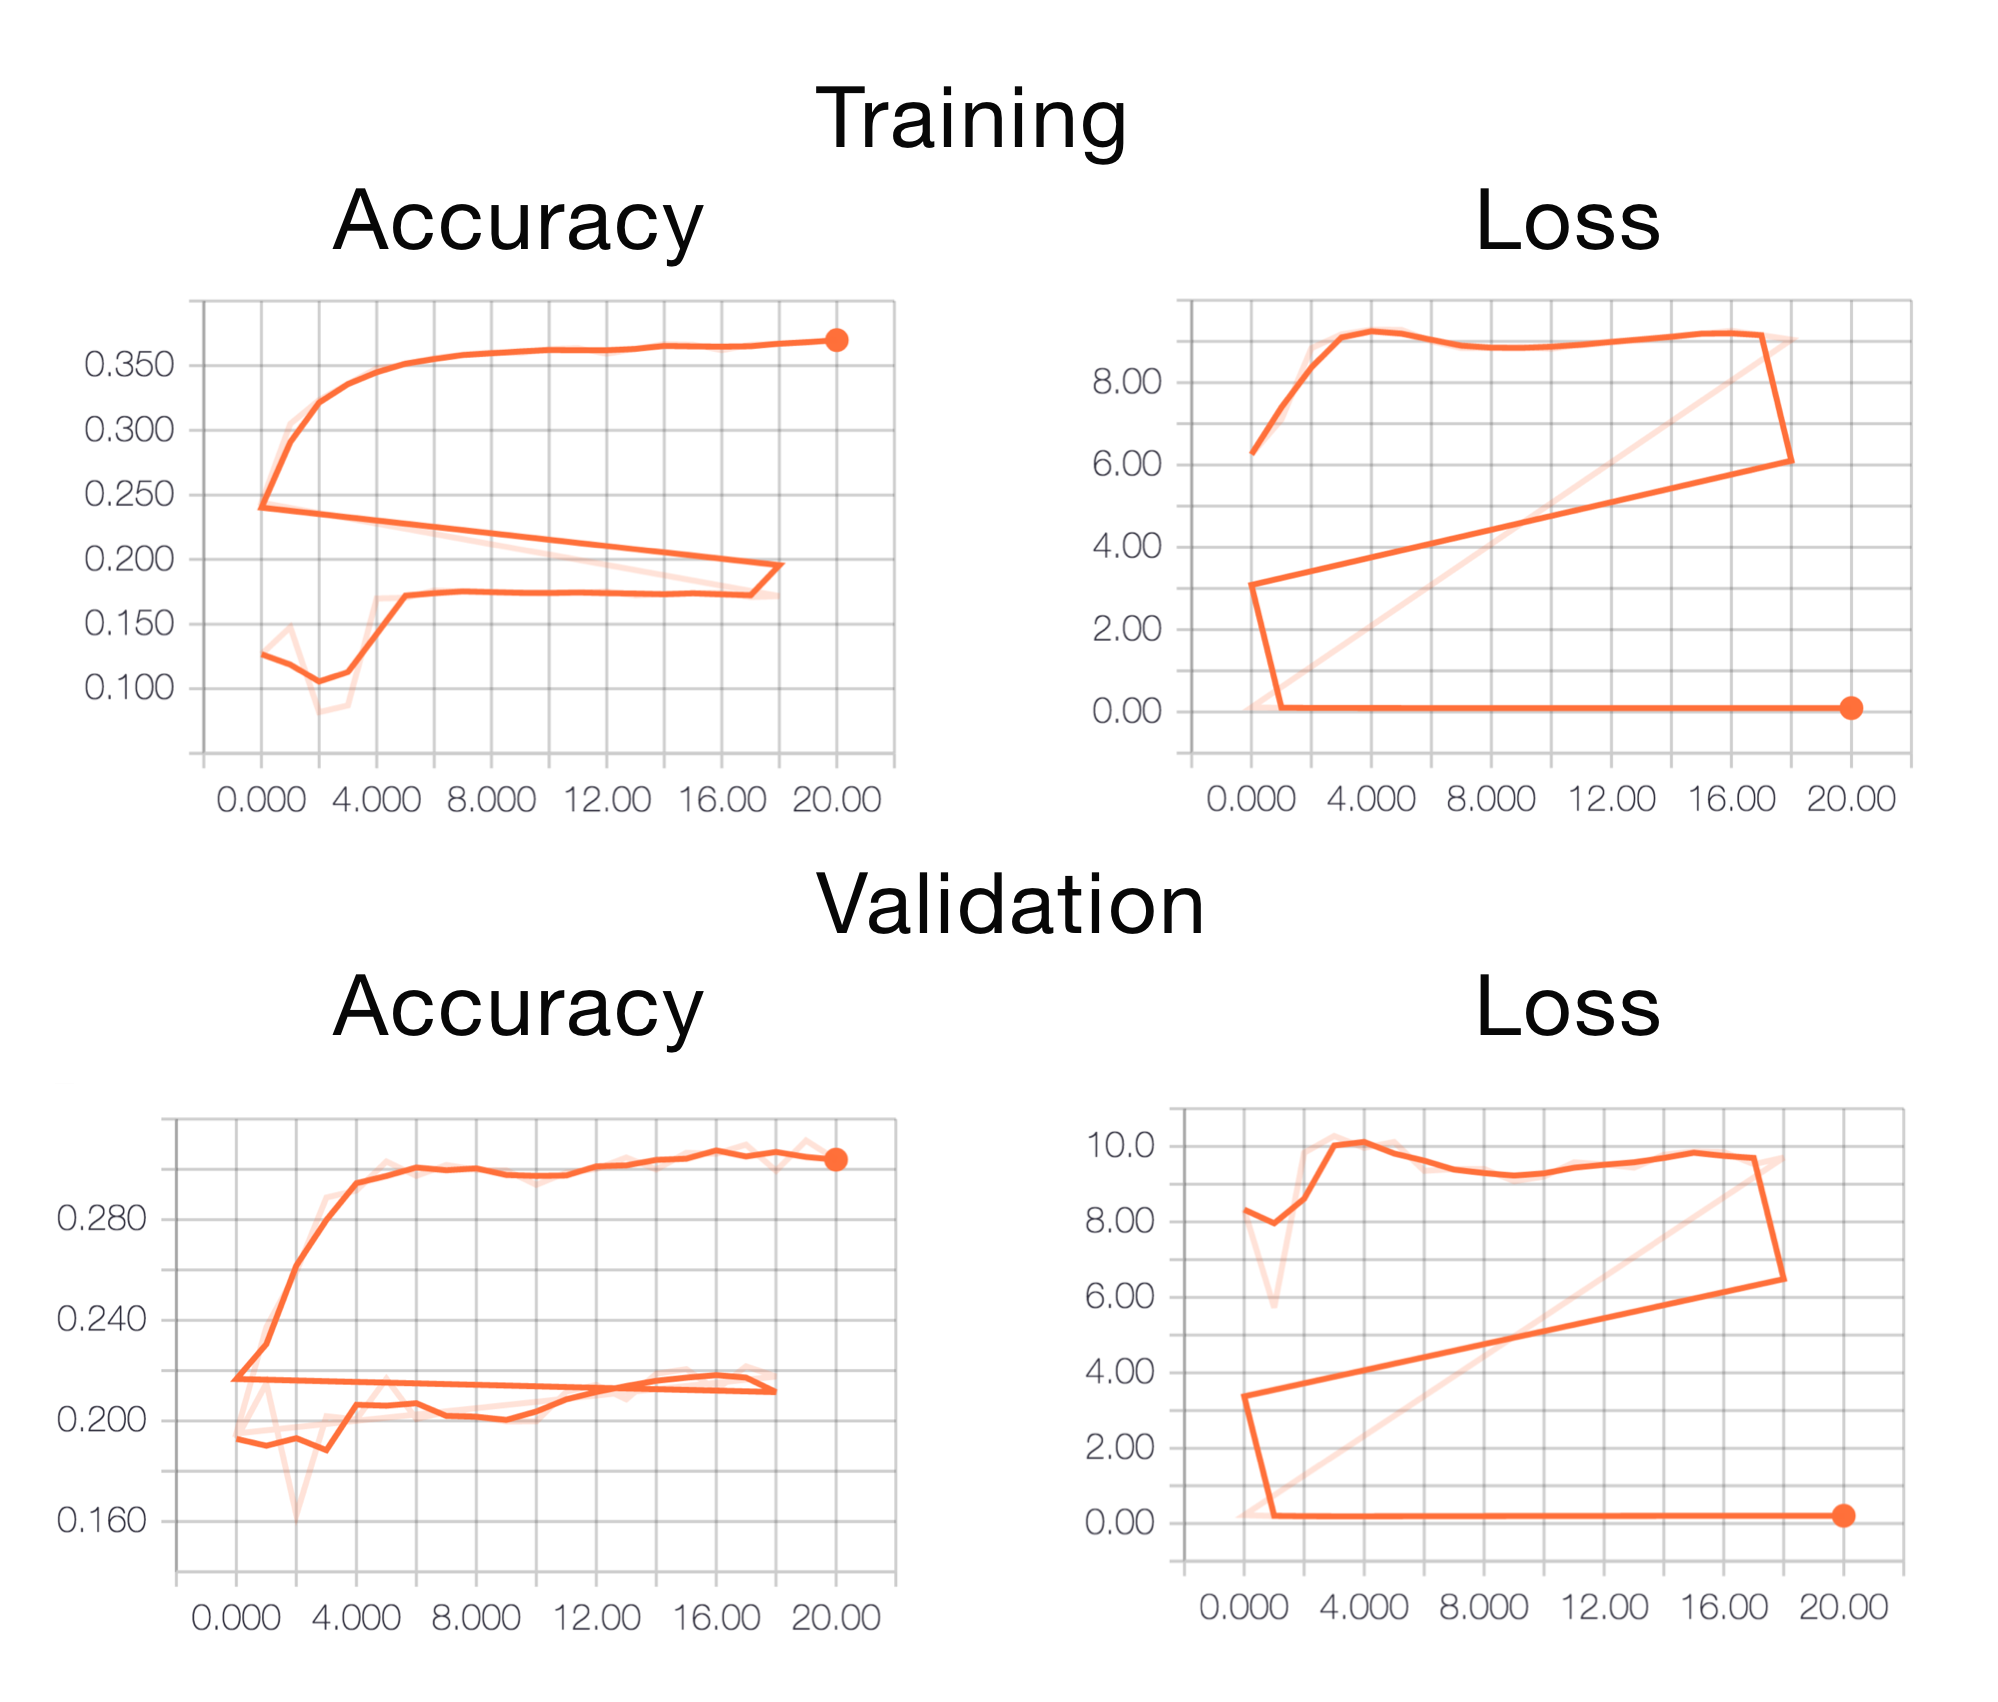
\includegraphics[width=0.7\textwidth,keepaspectratio]{length_fig}
	\caption{Fonéma hossz tanítás}
\end{figure}
\subsubsection{Teljes becslő}
A fenti paraméterek ismeretében teljes TTS végezhető. 

A mondat alapján fonéma hosszakat becslünk, majd párhuzamosan zöngésség-alapfrekvencia és mc paraméter becslés folyik, végül a kapott eredményekből előállítható a kimenet.
\clearpage
\subsection{Eredmények egy példán bemutatva}
Az alábbi {\it"But all my dreams violated this law"} mondaton elvégezve a becslést:
\subsubsection{Adatok beolvasása}
Az adatok beolvasása egy eredeti hangfájlból (\ref{law-1}.ábra), majd a csöndek szűrése és a pitch-MC paraméterek előállítása(\ref{law-2}.ábra).
\begin{figure}[h]
	
	\par\centering	
	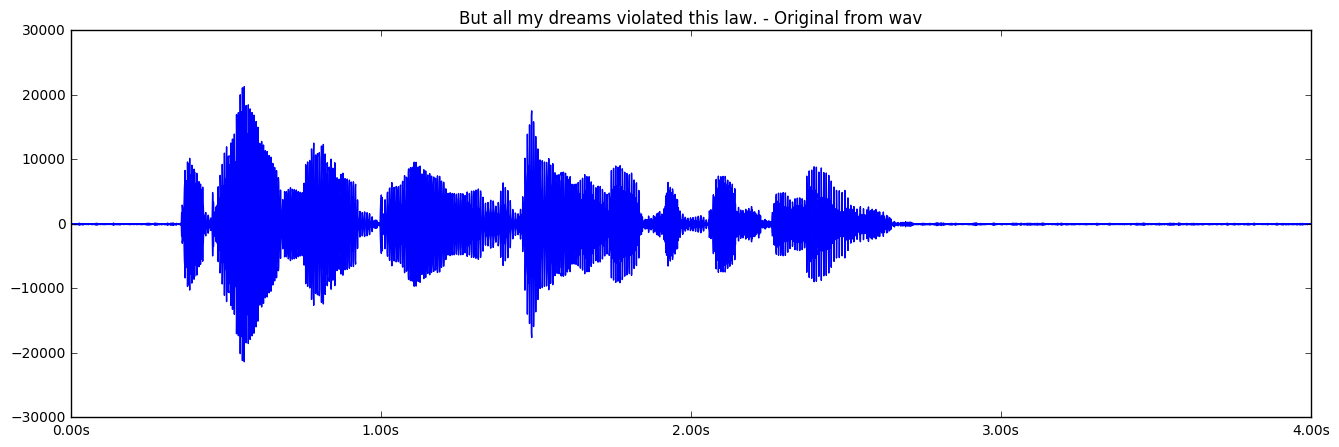
\includegraphics[width=\textwidth,keepaspectratio]{law_in}
	\caption{Beolvasott hangfájl}
	\label{law-1}
\end{figure}
\begin{figure}[h]
	\par\centering	
	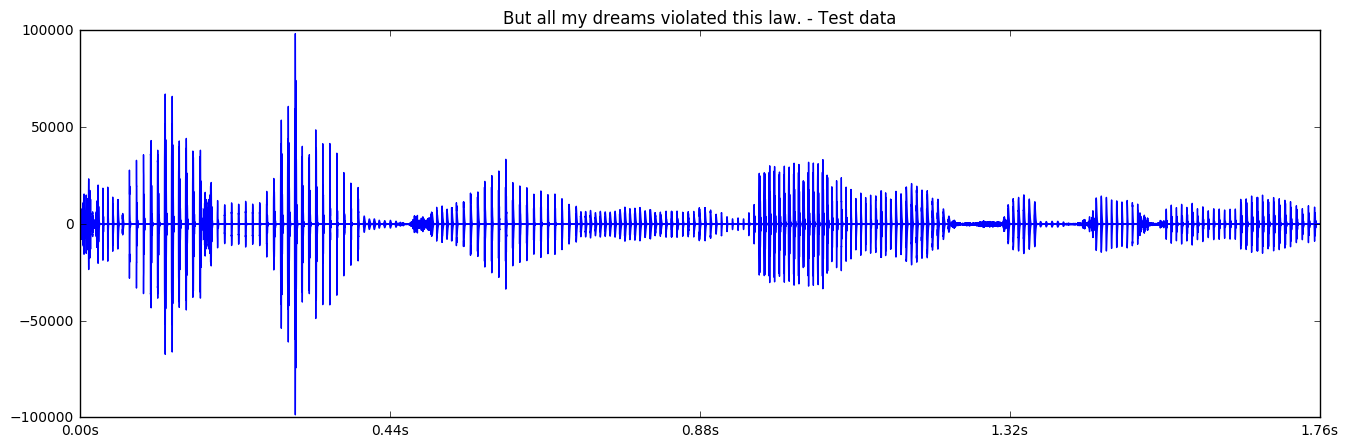
\includegraphics[width=\textwidth,keepaspectratio]{law_data}
	\caption{A hangfájl szűrve, MC-pitch értékek generálva PySPTK segítségével}
	\label{law-2}
\end{figure}
\subsubsection{Zöngésség becslés}
A zöngésség becslése jól működik.
\begin{figure}[h]
	
	\par\centering	
	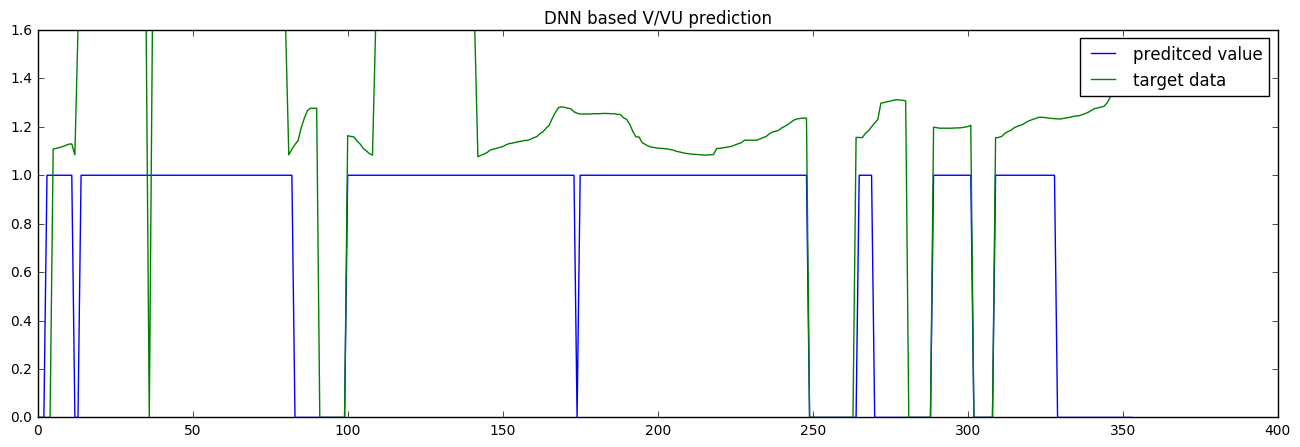
\includegraphics[width=\textwidth,keepaspectratio]{law_vuv}
	\caption{Beolvasott hangfájl}
\end{figure}
\subsubsection{Pitch becslés}
Alapfrekvencia becslése(\ref{law-3}. ábra), majd kimenet előállítása a tanult gerjesztési és a hozott spektrális paraméterekkel(\ref{law-4}. ábra). A \ref{law-5}. ábrán ugyanez látható a tanult zöngésség bevezetésével.
\begin{figure}[h]
	\par\centering	
	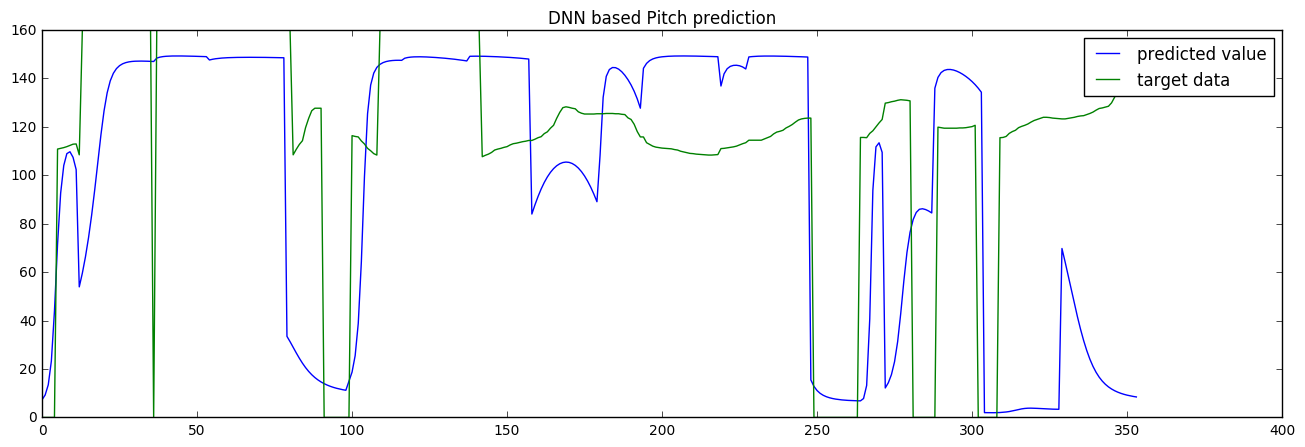
\includegraphics[width=\textwidth,keepaspectratio]{law_pitch}
	\caption{F0 becslése}
		\label{law-3}
\end{figure}
\begin{figure}[h]
	\par\centering	
	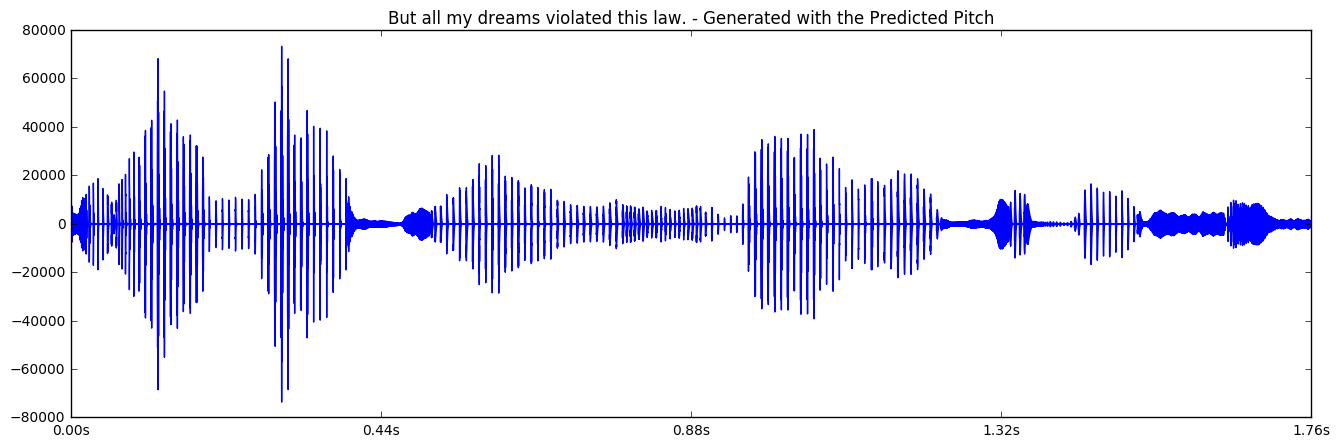
\includegraphics[width=\textwidth,keepaspectratio]{law_pitch_wav}
	\caption{Generált hang F0 becsléssel, MC az eredeti hang alapján}
		\label{law-4}
\end{figure}
\begin{figure}[h]
	\par\centering	
	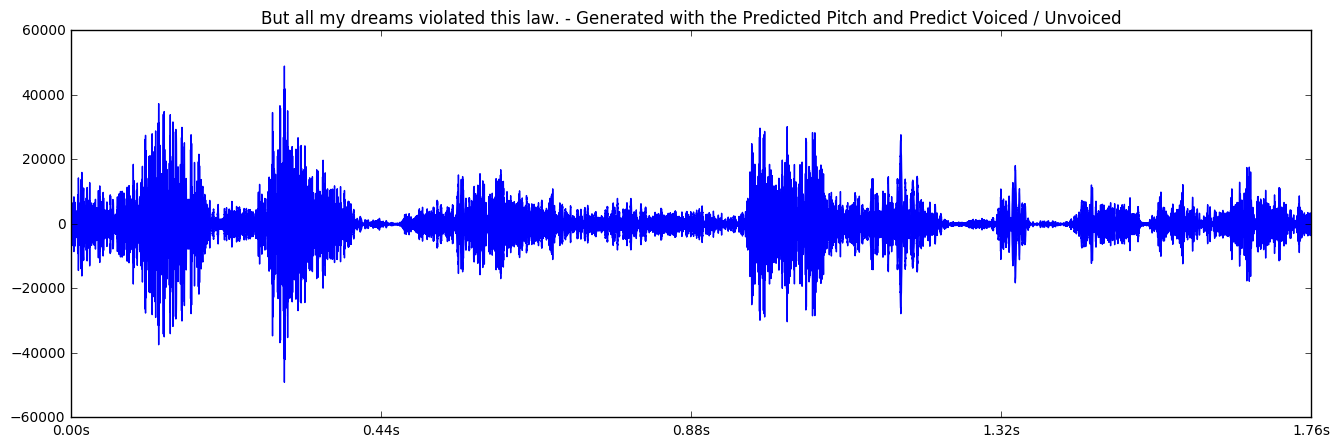
\includegraphics[width=\textwidth,keepaspectratio]{law_pitch_vuv}
	\caption{Generált hang F0 és V/UV értékek alapján}
		\label{law-5}
\end{figure}

\clearpage
\subsubsection{MC becslés}
Az MC becslőnél a görbe sajnos meglehetősen lépcsősen illeszkedik (\ref{law-6}. ábra), és ez a generált hangon is érezhető (\ref{law-7}. ábra).
\begin{figure}[h]
	\par\centering	
	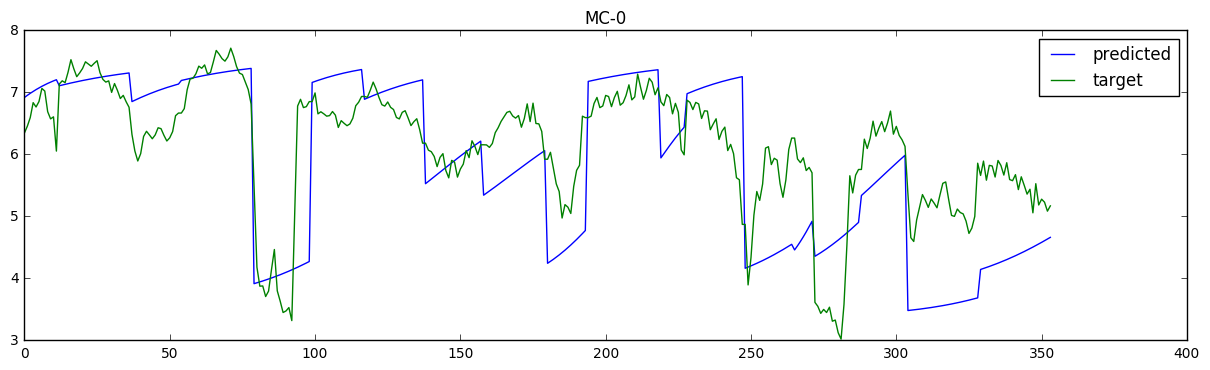
\includegraphics[width=\textwidth,keepaspectratio]{law_mc_0}
	\caption{MC-0 becslése}
	\label{law-6}
\end{figure}
\begin{figure}[h]
	\par\centering	
	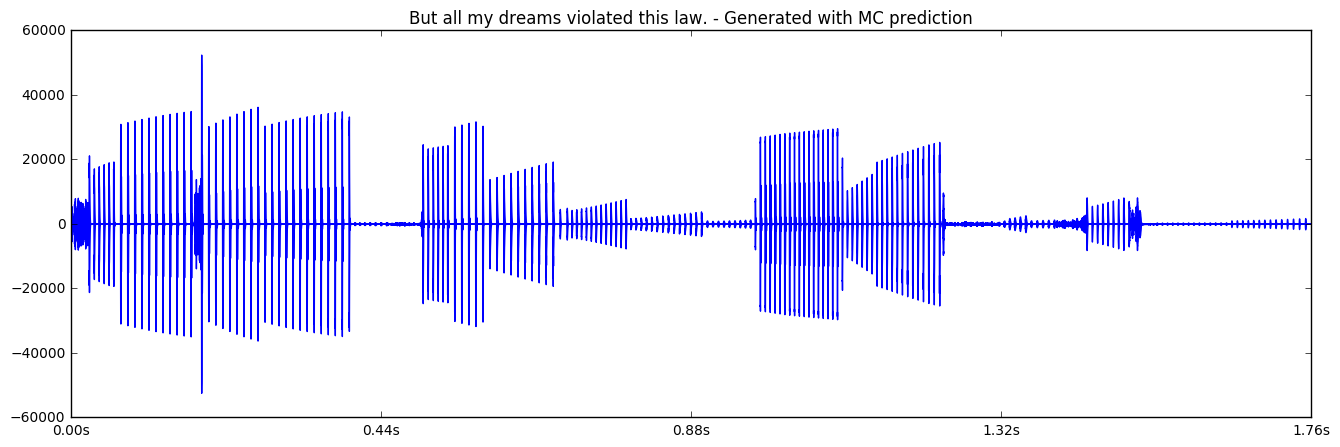
\includegraphics[width=\textwidth,keepaspectratio]{law_mc}
	\caption{Generált hang hozott F0-val és becsült MC értékekkel}
	\label{law-7}
\end{figure}
\subsubsection{Hanggenerálás tanult F0 és MC értékekkel}
A végleges generált hangból sajnos nem lehet kivenni az eredeti szavakat(\ref{law-8}. ábra).
\begin{figure}[h]
	\par\centering	
	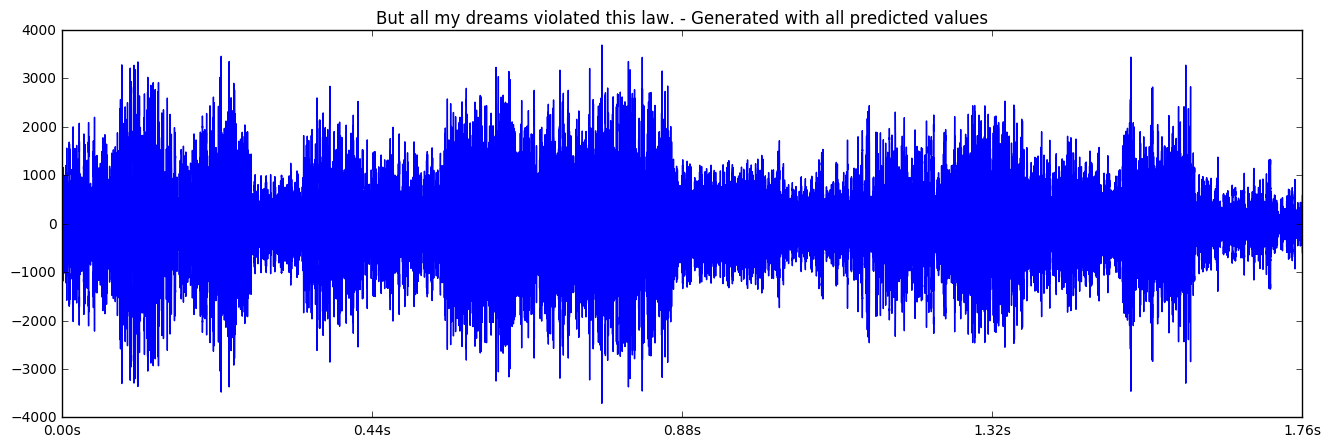
\includegraphics[width=\textwidth,keepaspectratio]{law_end}
	\caption{Generált hang becsült F0-val és MC értékekkel}
	\label{law-8}
\end{figure}
\chapter{}
\section{További lehetőségek}

A kész rendszerhez jelenleg két további problémát kell megoldanunk, egyrészt a fonémák hosszának becslésére külön új hálót kell létrehoznunk, valamint a spektrális paraméterek becslésén kell javítanunk. A hossz becslés egy új probléma ezzel még nem tudtunk foglalkozni, csak annyira hogy a generált tanító adatainkba szerepelnek már az ehhez tartozó elvárt értékek is. Spektrális paraméterek meghatározására már hoztunk létre és tanítottunk hálót, ennek pontosságán szeretnénk javítani. Az esetleges módszerek a következőek: további címkék létrehozása (pl. legyen több időkerettel kapcsolatos), más időfelbontás választása, más spektrális paraméter keresése.

A fenti bekezdés pontokban:

\begin{itemize}
	\item fonéma hossz becslése
	\item pontosabb spektrális paraméter becslés
	\item rendszer keretének megalkotása
\end{itemize}

Hosszútávú célként említhető még a WaveNet jellegű implementáció további fejlesztése.

\clearpage
\chapter{}
\section*{References}



\small

[1] Alexander, J.A.\ \& Mozer, M.C.\ (1995) Template-based algorithms
for connectionist rule extraction. In G.\ Tesauro, D.S.\ Touretzky and
T.K.\ Leen (eds.), {\it Advances in Neural Information Processing
  Systems 7}, pp.\ 609--616. Cambridge, MA: MIT Press.

[2] Bower, J.M.\ \& Beeman, D.\ (1995) {\it The Book of GENESIS:
  Exploring Realistic Neural Models with the GEneral NEural SImulation
  System.}  New York: TELOS/Springer--Verlag.

[3] Hasselmo, M.E., Schnell, E.\ \& Barkai, E.\ (1995) Dynamics of
learning and recall at excitatory recurrent synapses and cholinergic
modulation in rat hippocampal region CA3. {\it Journal of
  Neuroscience} {\bf 15}(7):5249-5262.
\chapter{}
\subsubsection*{Köszönetnyilvánítás}

A dokumentum és a szerzők munkái nagyban támaszkodnak a Budapesti Műszaki és Gazdaságtudományi Egyetemen tartott Deep Learning a gyakorlatban Python és LUA alapokon tárgy keretei között elhangzott információkra


\end{document}
